%***************************************************************************************
\section{Prior Uncertainty Propagation of the FEBA Tests}\label{app:tbl_results_uq_feba}
%***************************************************************************************

%--------------------------------------------------------------------------
\subsection{Clad Temperature Output (TC)}\label{app:tbl_results_uq_feba_tc}
%--------------------------------------------------------------------------

% FEBA test no. 214 Prior Uncertainty Propagation, TC
\rotatebox{90}{\begin{minipage}{0.75\textheight}
    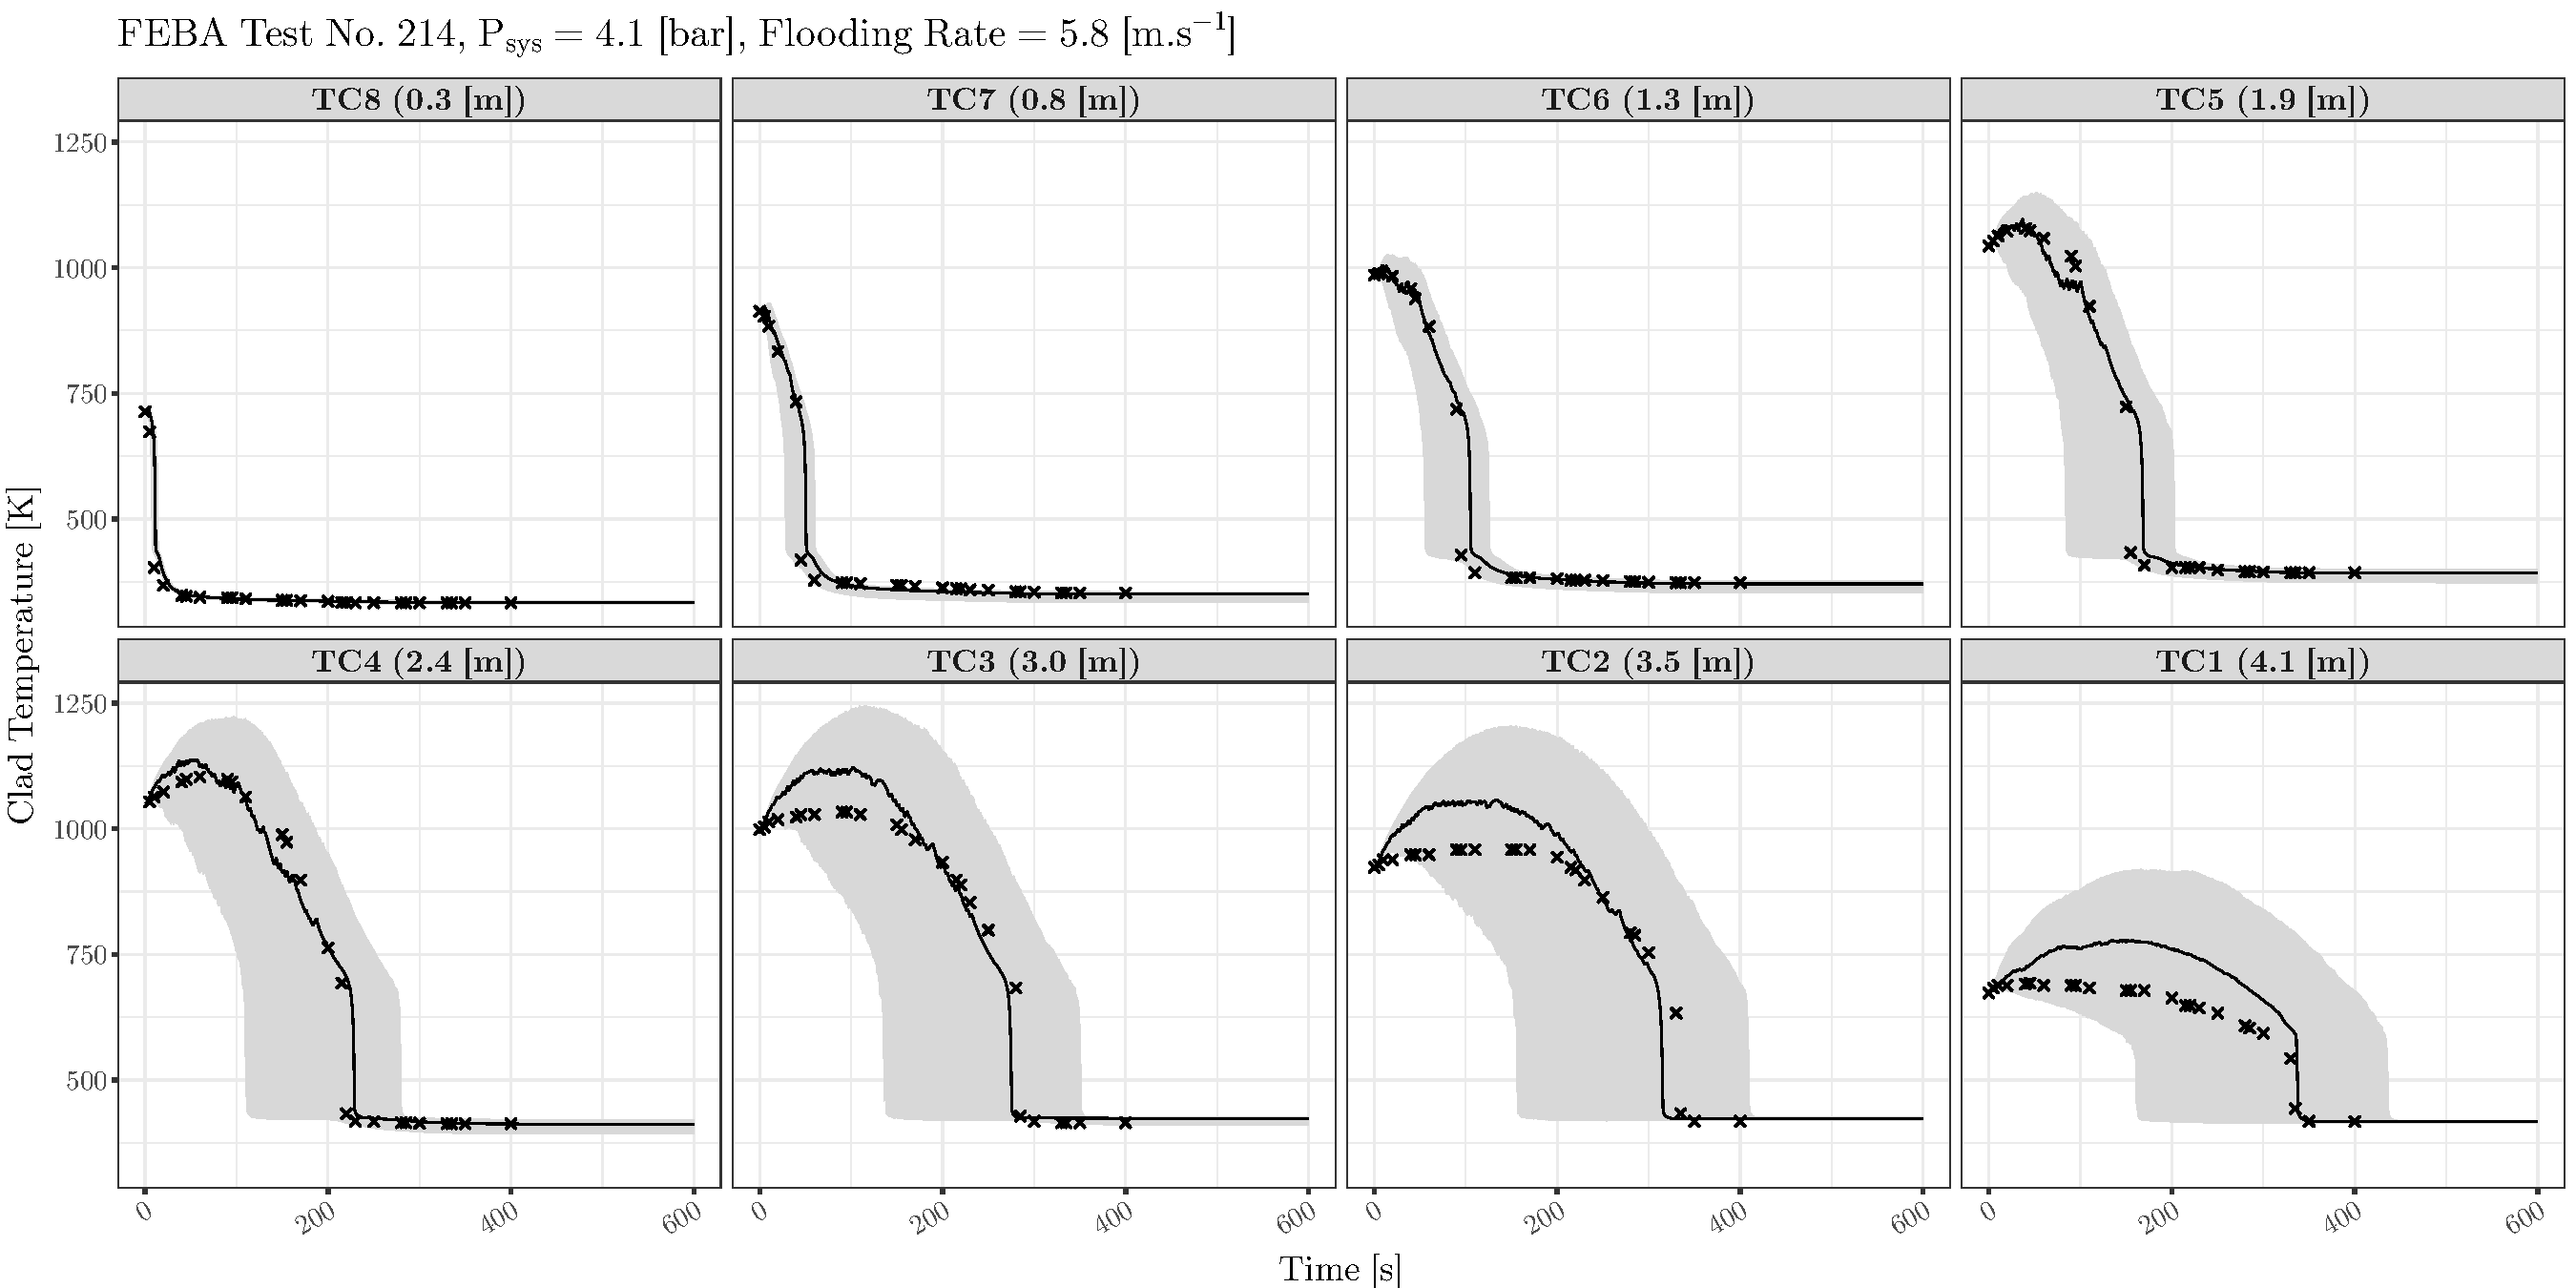
\includegraphics[width=1\textwidth]{../figures/chapter2/figures/plotTraceUQPriorTC214}
		\captionof{figure}[Propagation of the $27$ input parameters prior uncertainties on FEBA test no. $214$ for the clad temperature output ($TC$).]{Propagation of the $27$ input parameters prior uncertainties on FEBA test no. $214$ for the clad temperature output ($TC$) at different axial locations using \gls[hyper=false]{trace}. The uncertainty bounds correspond to the symmetric ($95\%$) probability; solid lines and crosses indicate the simulation with the nominal parameters values and the experimental data, respectively.}
    \label{fig:ch2_plot_trace_uq_prior_tc_214}
\end{minipage}}

% FEBA test no. 216 Prior Uncertainty Propagation, TC
\clearpage
\begin{sidewaysfigure}
	\centering
	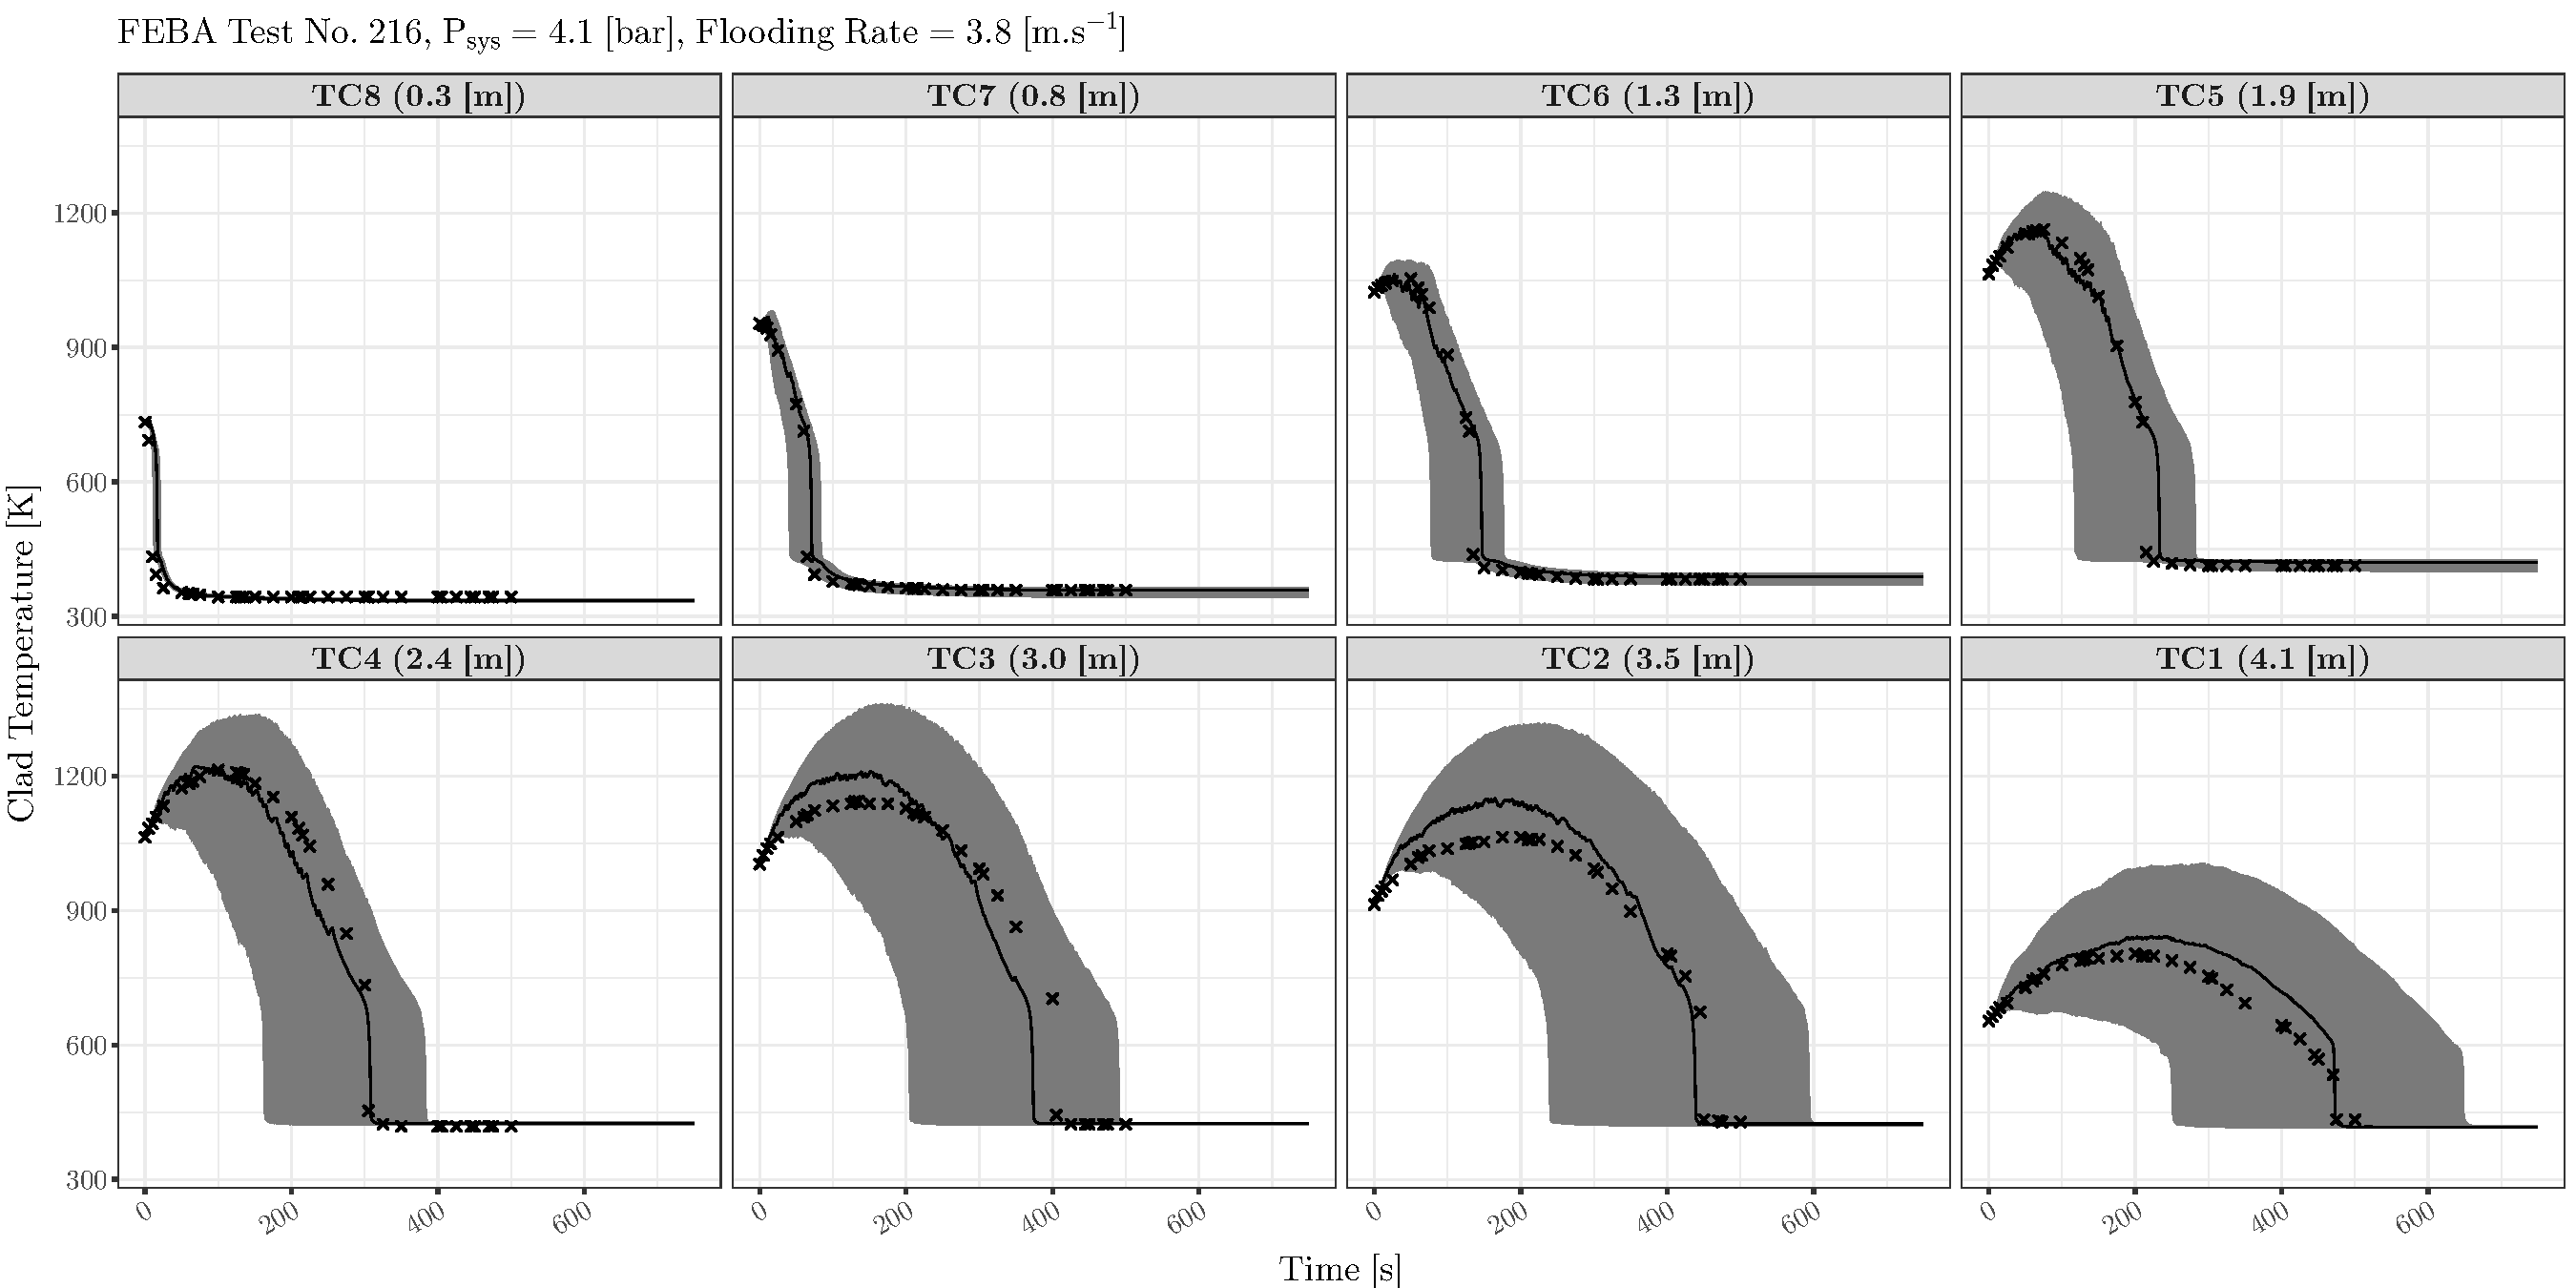
\includegraphics[width=1.0\textwidth]{../figures/chapter2/figures/plotTraceUQPriorTC216}
		\captionof{figure}[Propagation of the $27$ input parameters prior uncertainties on FEBA test no. $216$ for the clad temperature output ($TC$).]{Propagation of the $27$ input parameters prior uncertainties on FEBA test no. $216$ for the clad temperature output ($TC$) at different axial locations using \gls[hyper=false]{trace}. The uncertainty bounds correspond to the symmetric ($95\%$) probability; solid lines and crosses indicate the simulation with the nominal parameters values and the experimental data, respectively.}
	\label{fig:ch2_app_plot_trace_uq_prior_tc_216}
\end{sidewaysfigure}
\clearpage

% FEBA test no. 223 Prior Uncertainty Propagation, TC
\clearpage
\begin{sidewaysfigure}
	\centering
	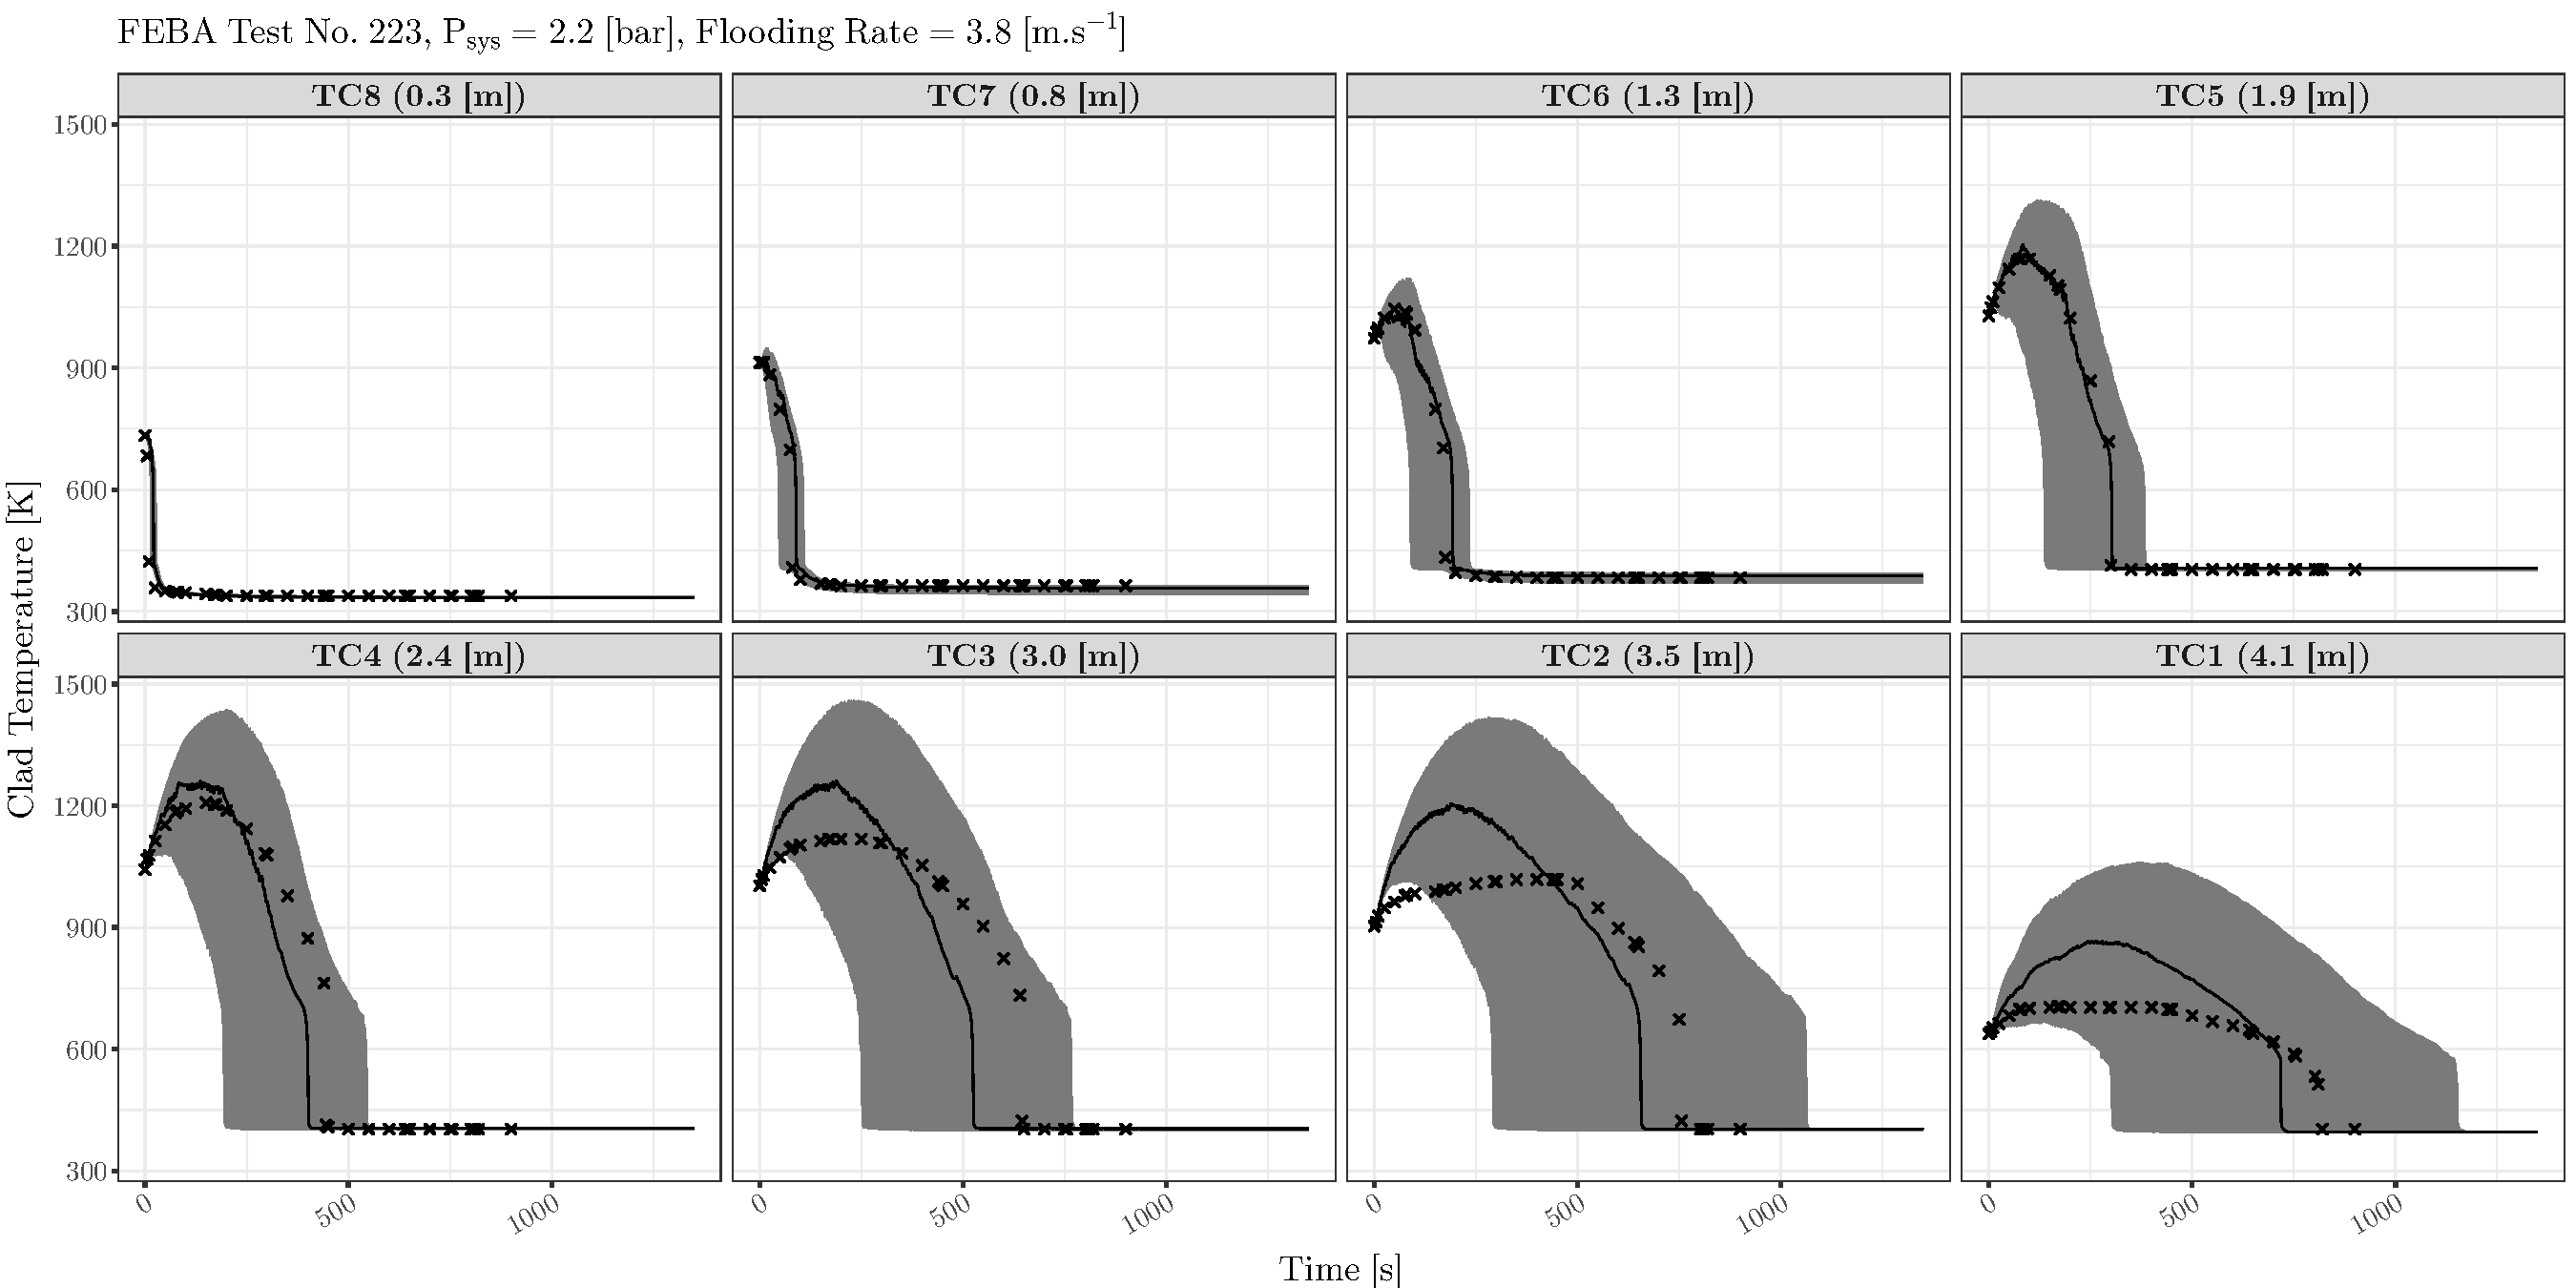
\includegraphics[width=1.0\textwidth]{../figures/chapter2/figures/plotTraceUQPriorTC223}
		\captionof{figure}[Propagation of the $27$ input parameters prior uncertainties on FEBA test no. $223$ for the clad temperature output ($TC$).]{Propagation of the $27$ input parameters prior uncertainties on FEBA test no. $223$ for the clad temperature output ($TC$) at different axial locations using \gls[hyper=false]{trace}. The uncertainty bounds correspond to the symmetric ($95\%$) probability; solid lines and crosses indicate the simulation with the nominal parameters values and the experimental data, respectively.}
	\label{fig:ch2_plot_trace_uq_prior_tc_223}
\end{sidewaysfigure}
\clearpage

% FEBA test no. 218 Prior Uncertainty Propagation, TC
\clearpage
\begin{sidewaysfigure}
	\centering
	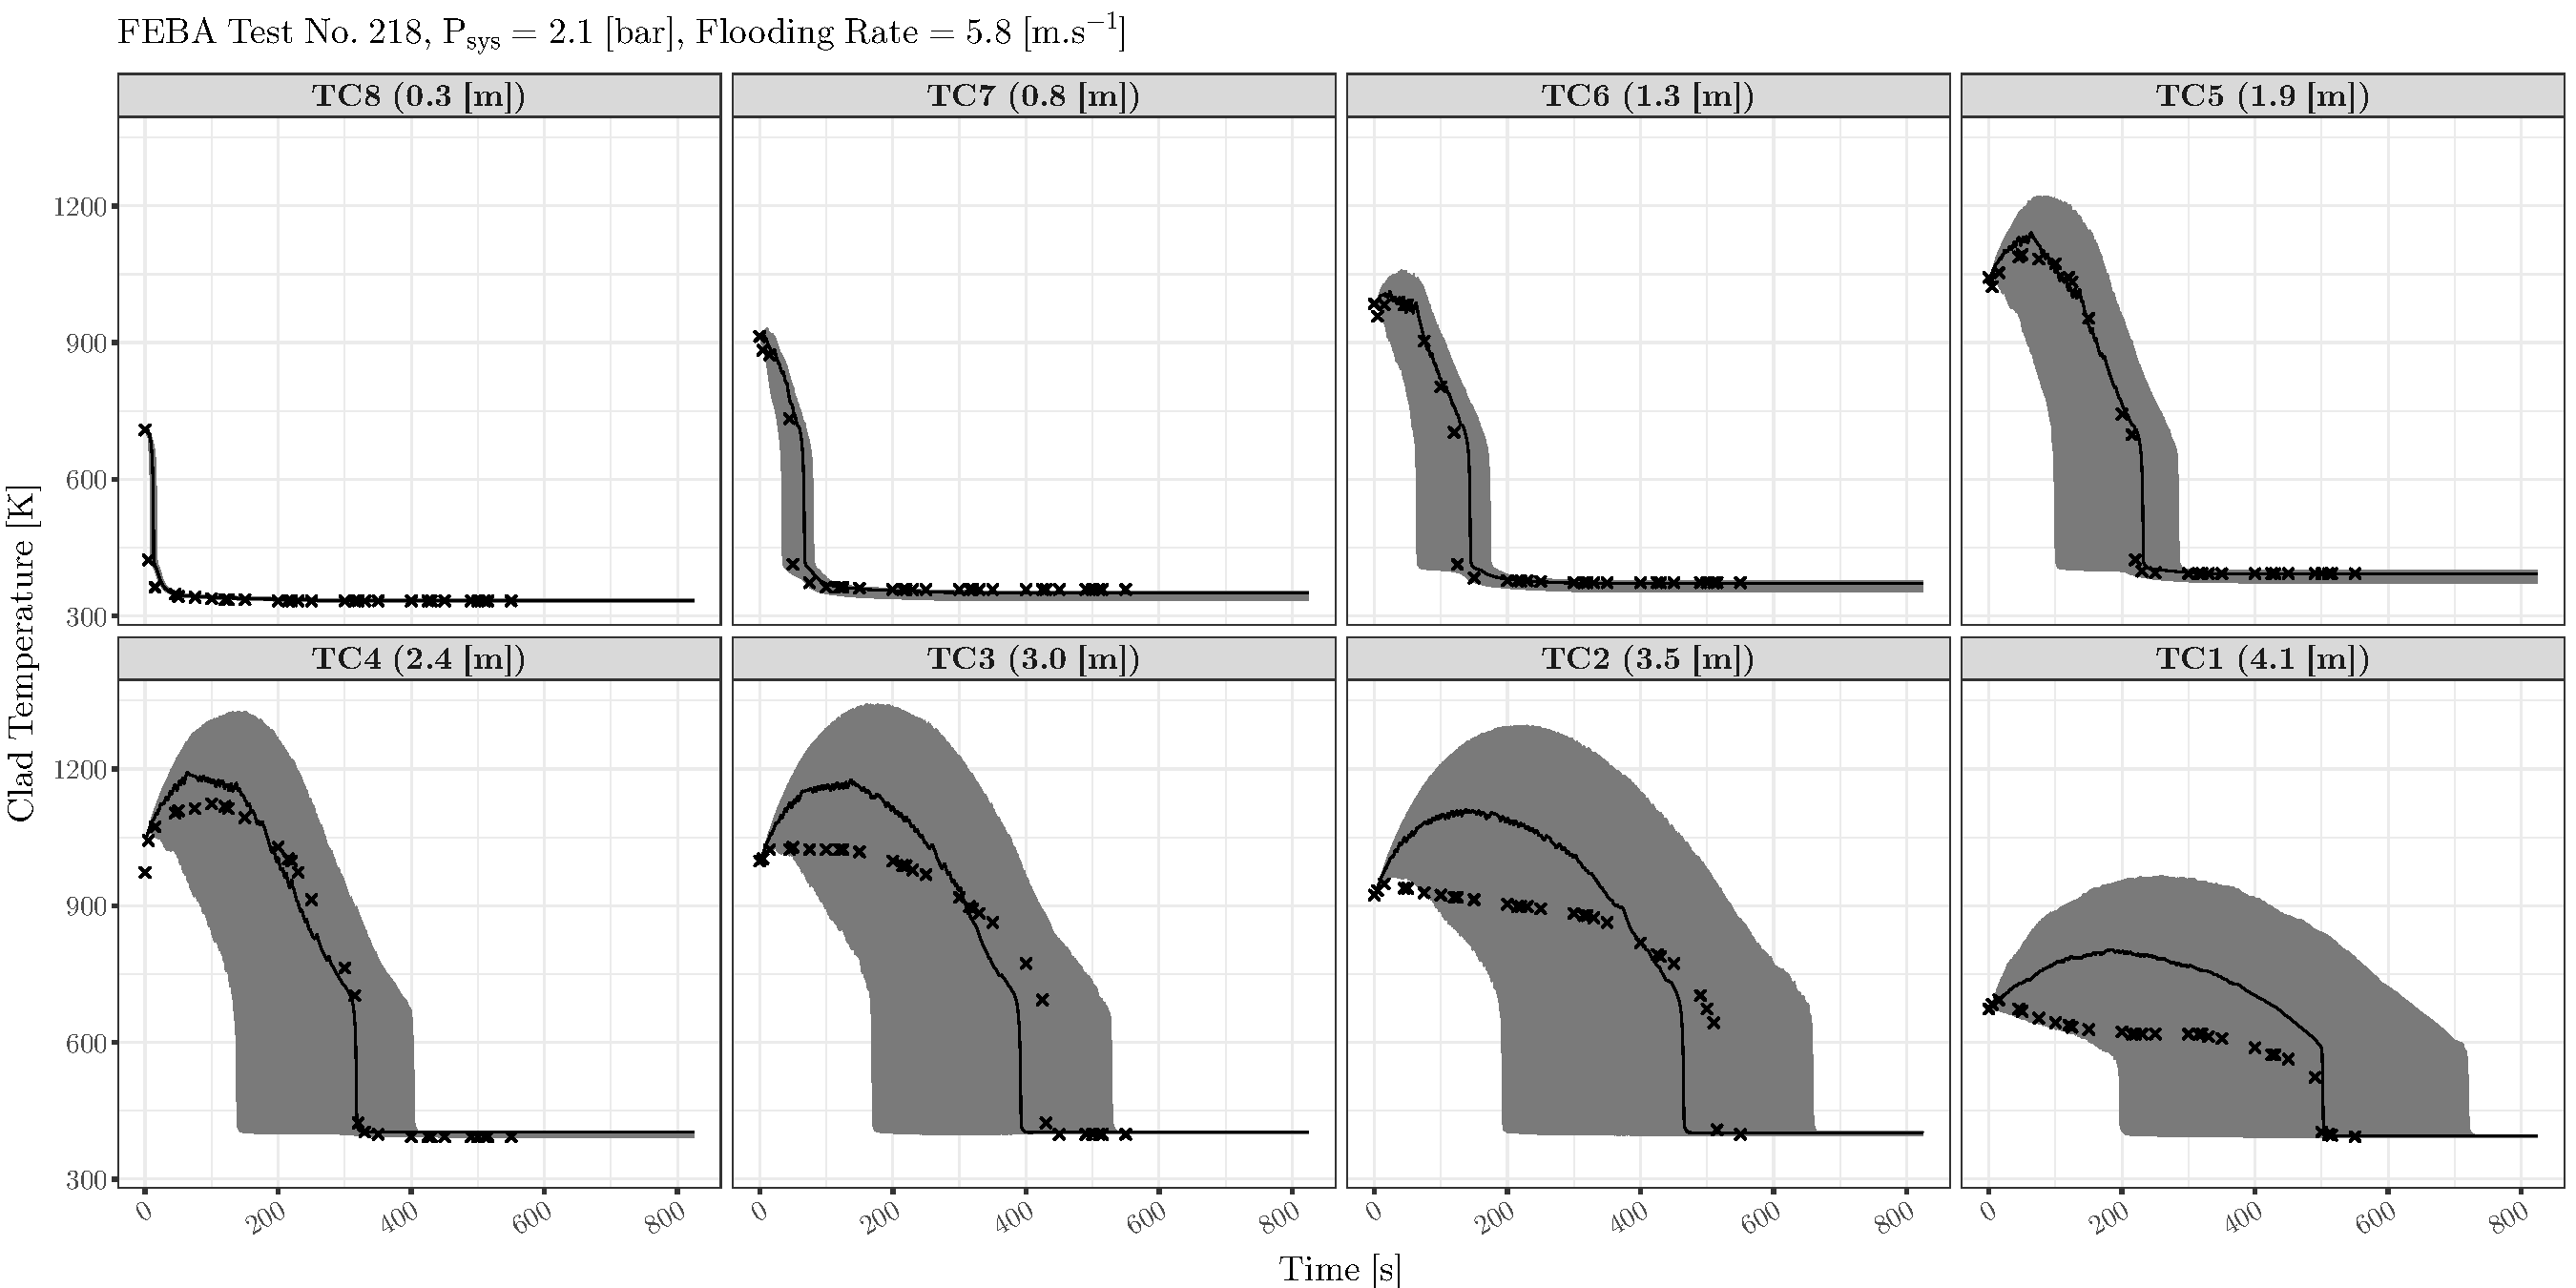
\includegraphics[width=1.0\textwidth]{../figures/chapter2/figures/plotTraceUQPriorTC218}
		\captionof{figure}[Propagation of the $27$ input parameters prior uncertainties on FEBA test no. $218$ for the clad temperature output ($TC$).]{Propagation of the $27$ input parameters prior uncertainties on FEBA test no. $218$ for the clad temperature output ($TC$) at different axial locations using \gls[hyper=false]{trace}. The uncertainty bounds correspond to the symmetric ($95\%$) probability; solid lines and crosses indicate the simulation with the nominal parameters values and the experimental data, respectively.}
	\label{fig:ch2_plot_trace_uq_prior_tc_218}
\end{sidewaysfigure}
\clearpage

% FEBA test no. 220 Prior Uncertainty Propagation, TC
\clearpage
\begin{sidewaysfigure}
	\centering
	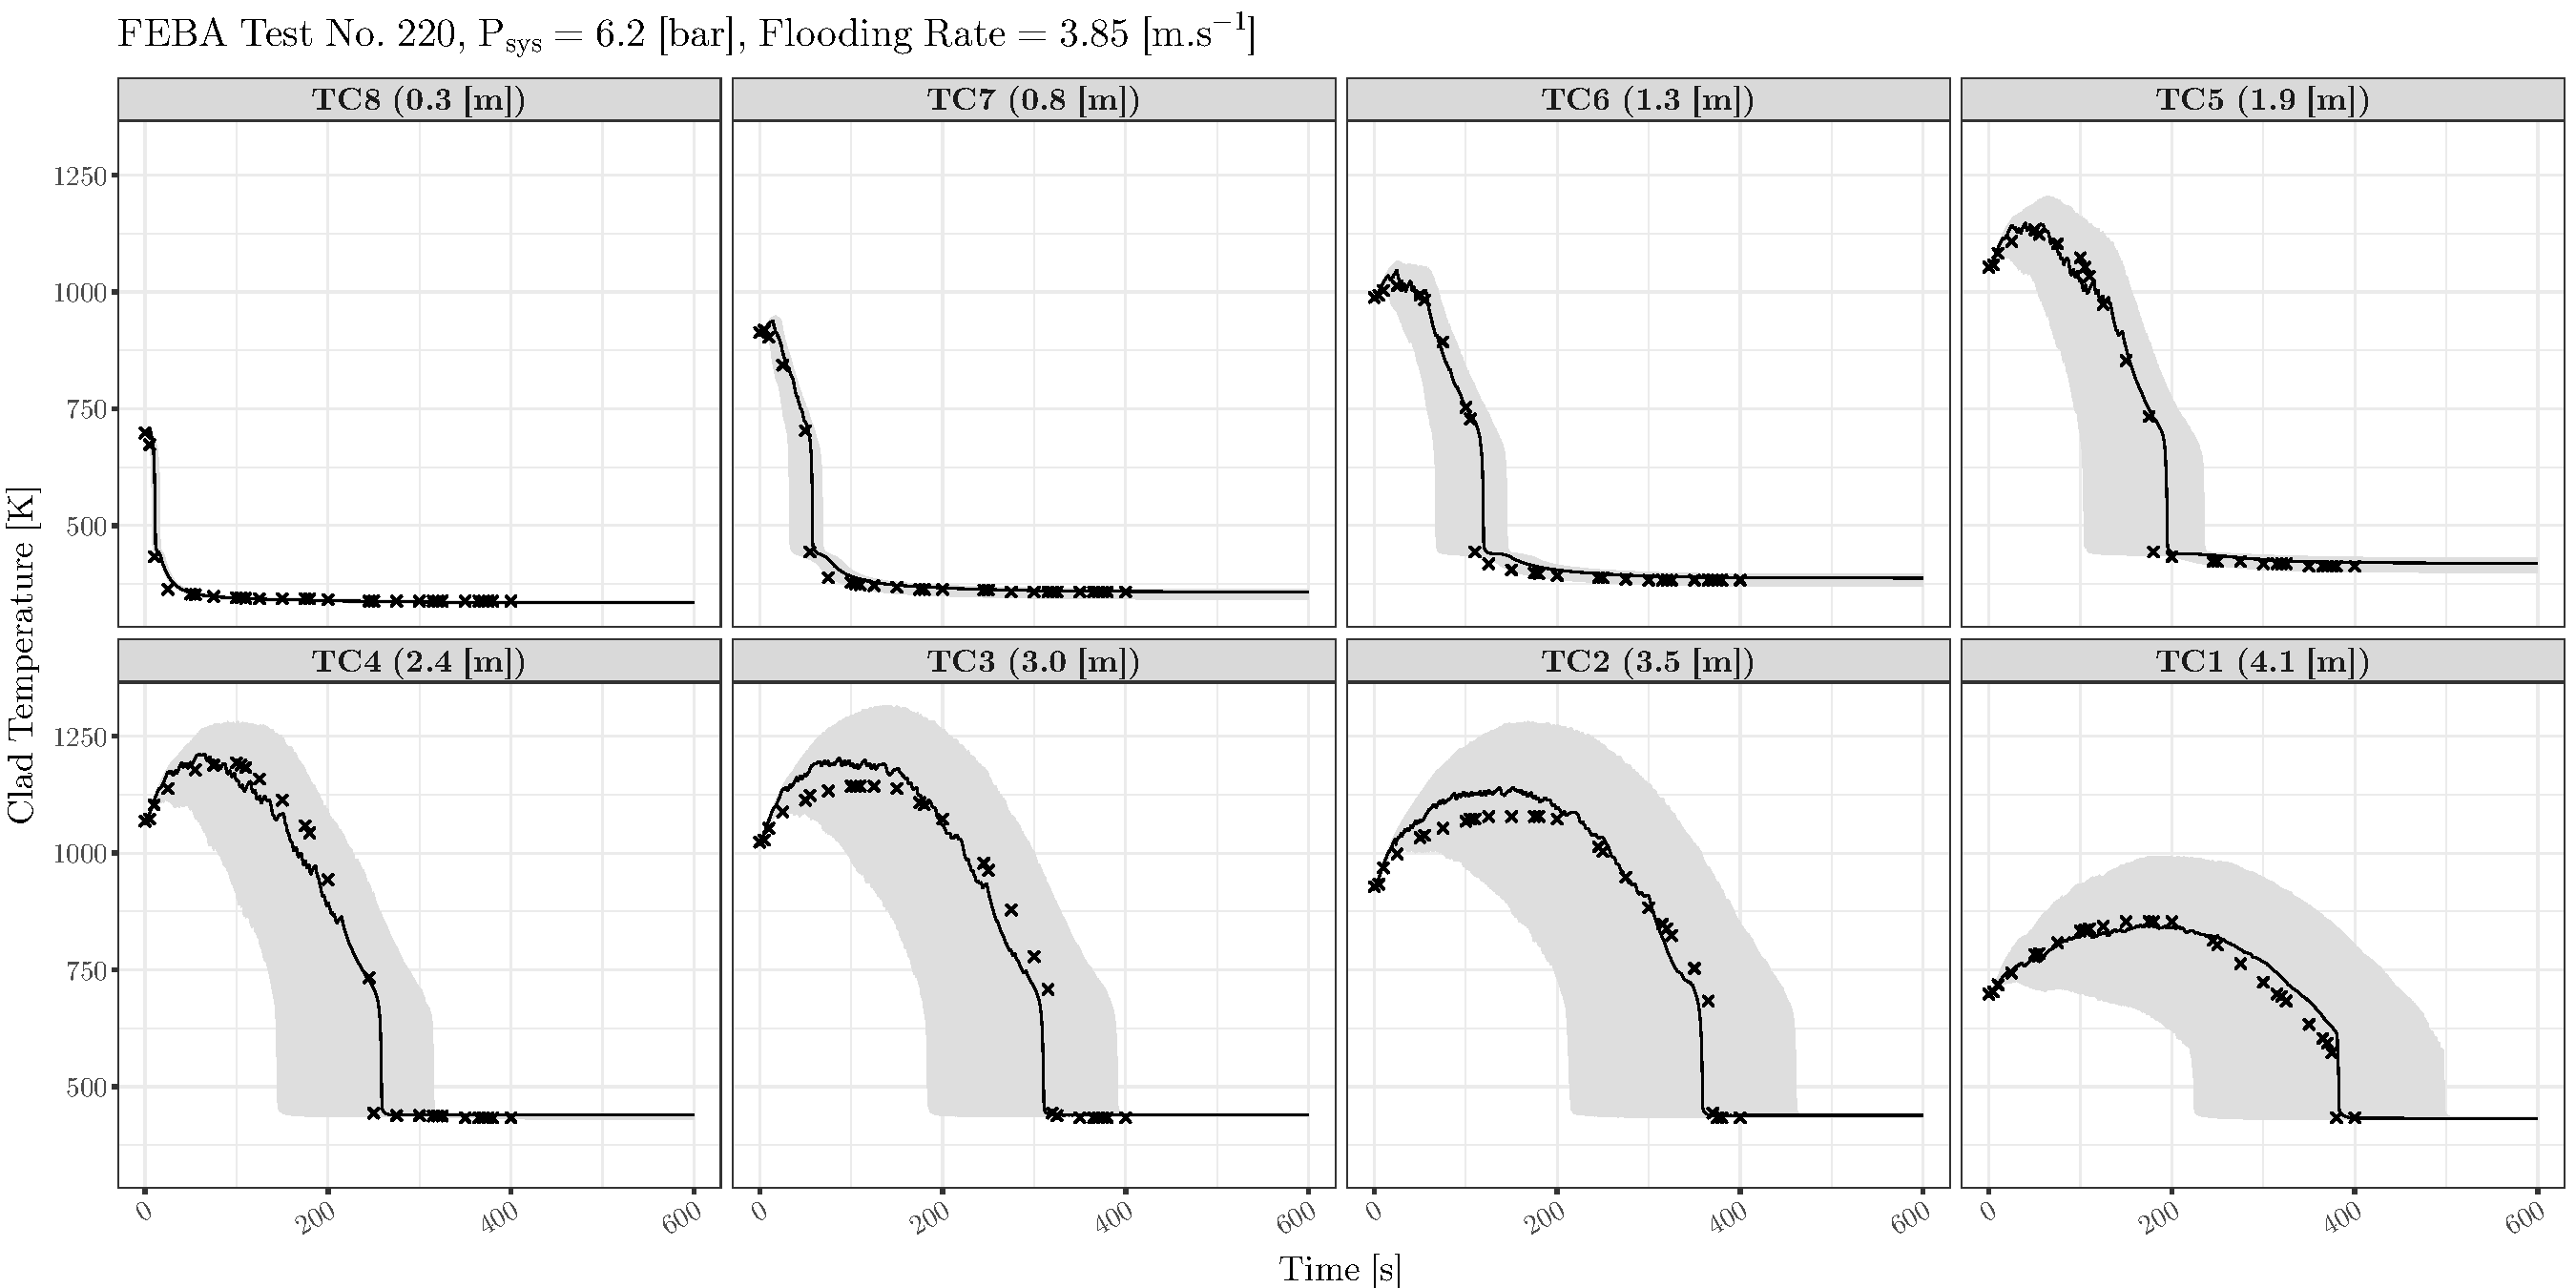
\includegraphics[width=1.0\textwidth]{../figures/chapter2/figures/plotTraceUQPriorTC220}
		\captionof{figure}[Propagation of the $27$ input parameters prior uncertainties on FEBA test no. $220$ for the clad temperature output ($TC$).]{Propagation of the $27$ input parameters prior uncertainties on FEBA test no. $220$ for the clad temperature output ($TC$) at different axial locations using \gls[hyper=false]{trace}. The uncertainty bounds correspond to the symmetric ($95\%$) probability; solid lines and crosses indicate the simulation with the nominal parameters values and the experimental data, respectively.}
	\label{fig:ch2_plot_trace_uq_prior_tc_220}
\end{sidewaysfigure}
\clearpage

% FEBA test no. 222 Prior Uncertainty Propagation, TC
\clearpage
\begin{sidewaysfigure}
	\centering
	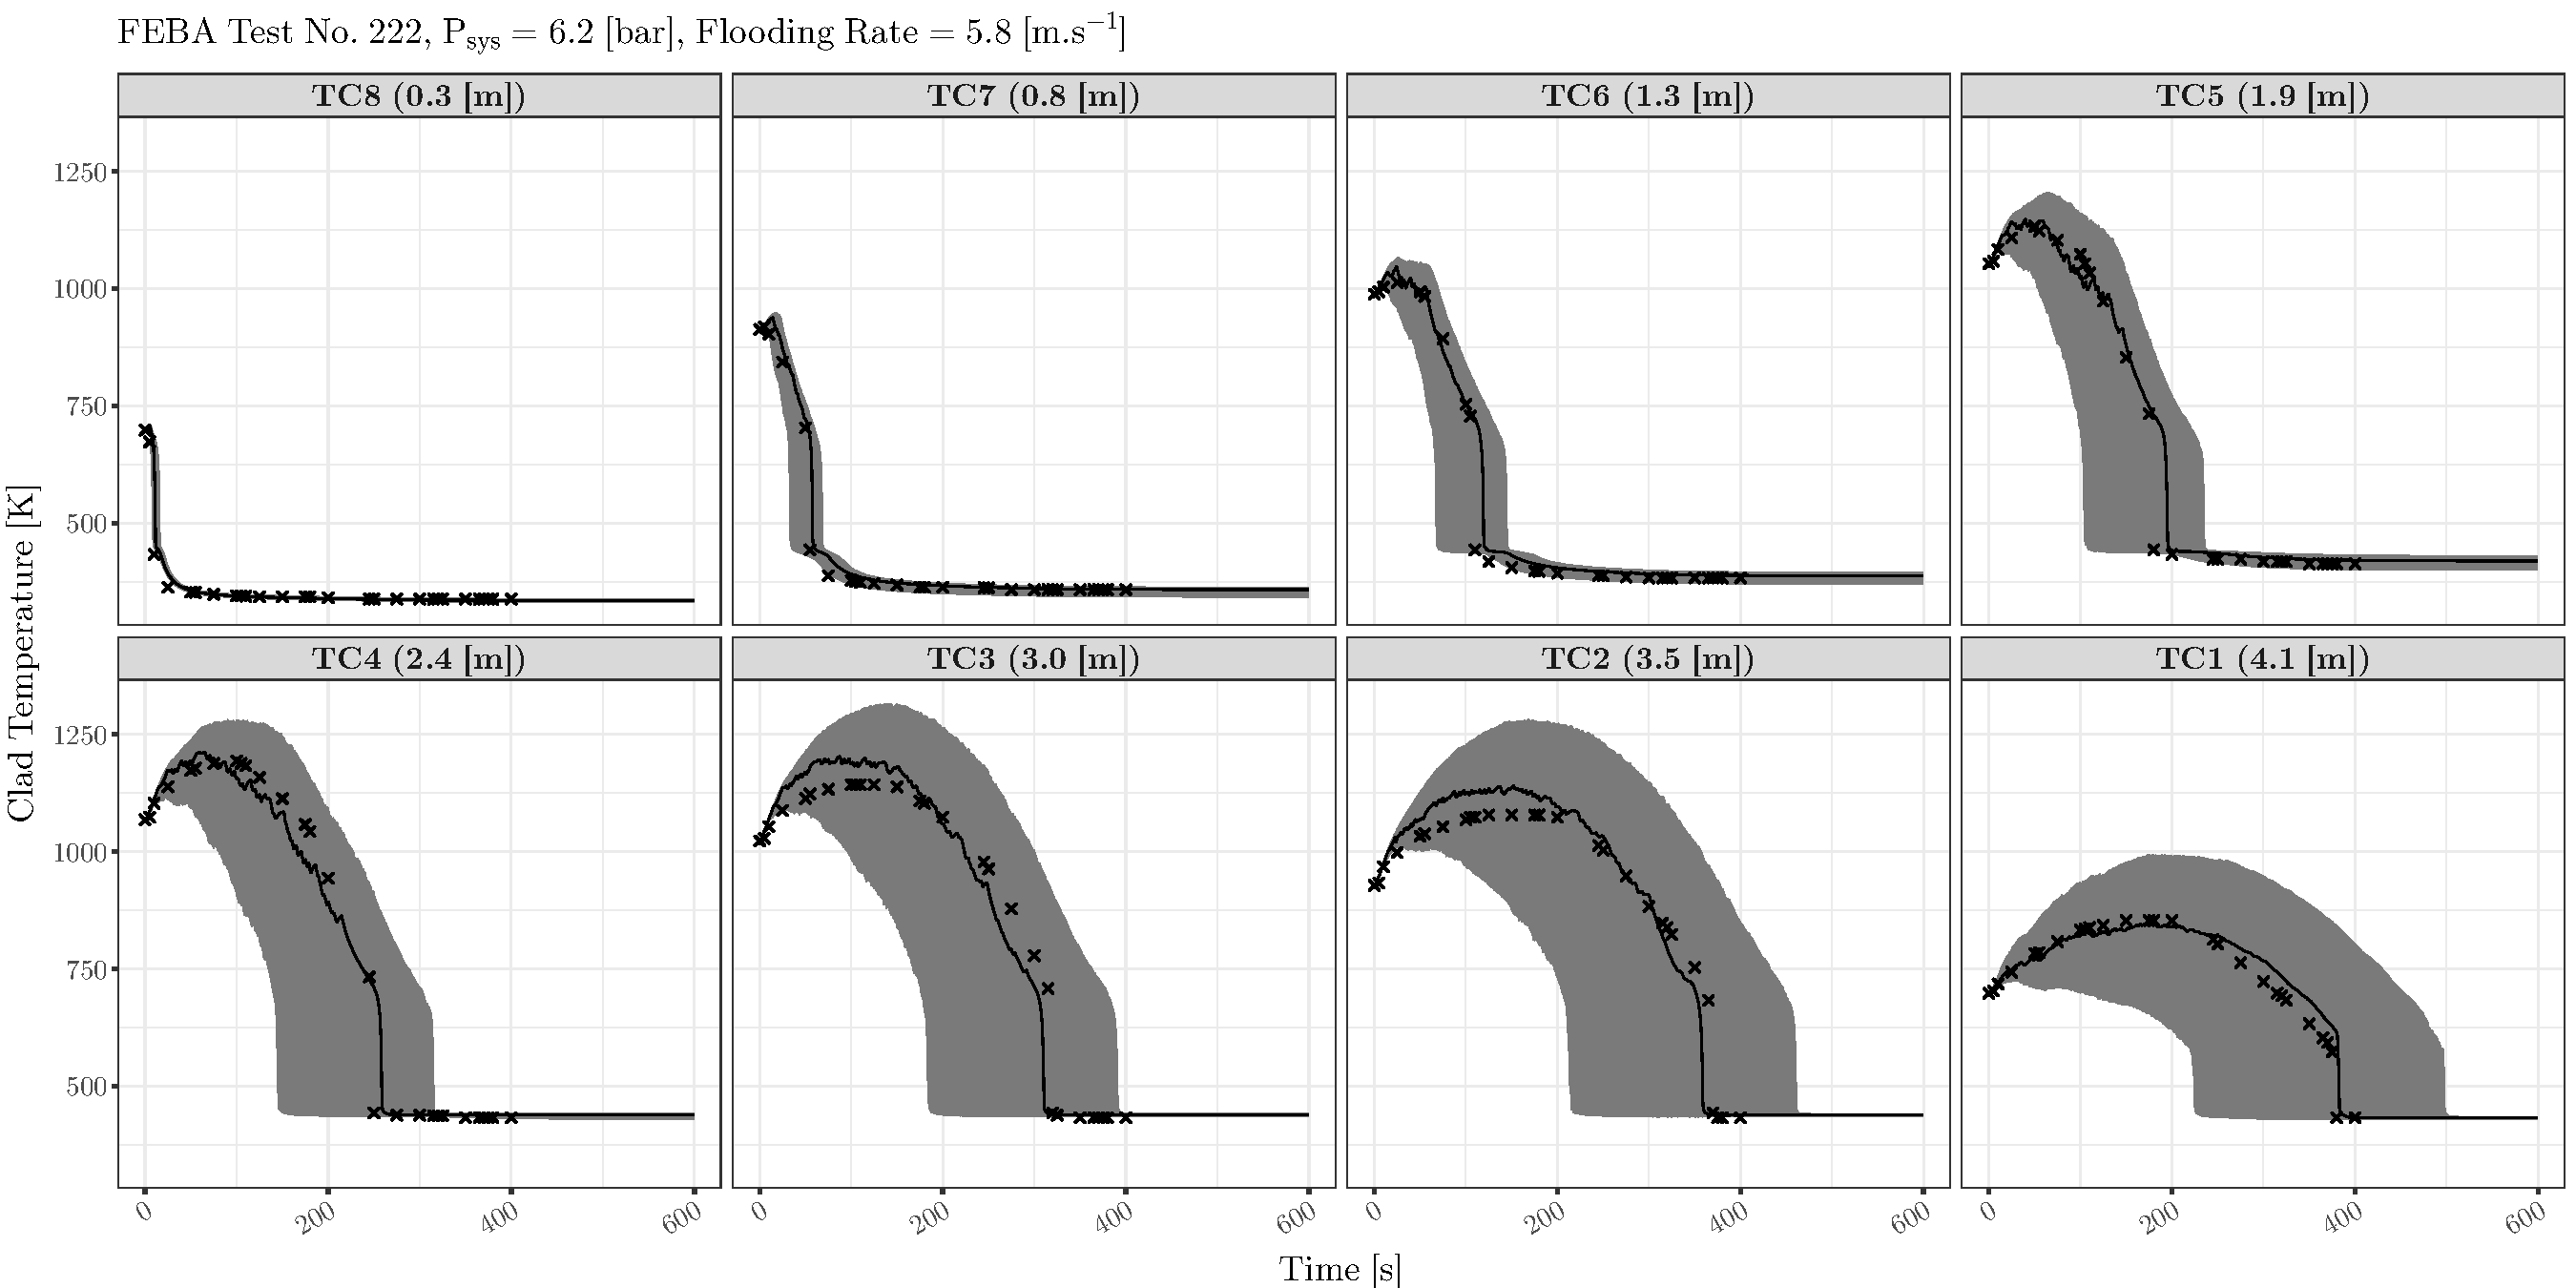
\includegraphics[width=1.0\textwidth]{../figures/chapter2/figures/plotTraceUQPriorTC222}
		\captionof{figure}[Propagation of the $27$ input parameters prior uncertainties on FEBA test no. $222$ for the clad temperature output ($TC$).]{Propagation of the $27$ input parameters prior uncertainties on FEBA test no. $222$ for the clad temperature output ($TC$) at different axial locations using \gls[hyper=false]{trace}. The uncertainty bounds correspond to the symmetric ($95\%$) probability; solid lines and crosses indicate the simulation with the nominal parameters values and the experimental data, respectively.}
	\label{fig:ch2_plot_trace_uq_prior_tc_222}
\end{sidewaysfigure}
\clearpage

%-----------------------------------------------------------------------
\subsection{Pressure Drop Output (DP)}\label{app:tbl_results_uq_feba_dp}
%-----------------------------------------------------------------------

% FEBA test no. 214 Prior Uncertainty Propagation, DP
\begin{figure}[bth]
    \centering
    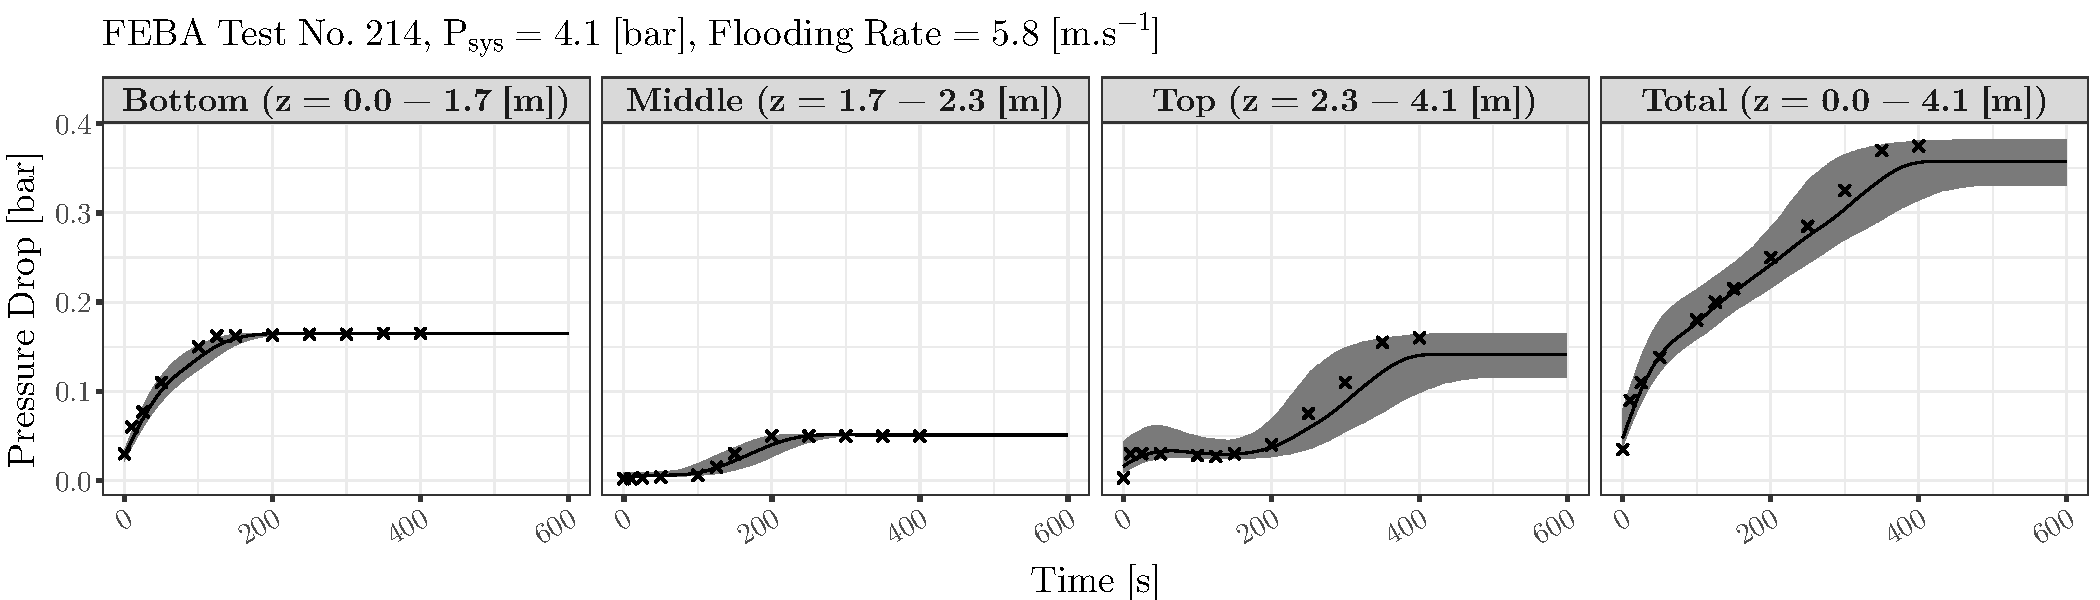
\includegraphics[width=1.0\textwidth]{../figures/chapter2/figures/plotTraceUQPriorDP214}
    \caption[Propagation of the $27$ input parameters prior uncertainties on FEBA test no. $214$ for the pressure drop output ($DP$).]{Propagation of the $27$ input parameters prior uncertainties on FEBA test no. $214$ for the pressure drop output ($DP$). The uncertainty bounds correspond to the symmetric ($95\%$) probability; solid lines and crosses indicate the simulation with the nominal parameters values and the experimental data, respectively.}
    \label{fig:ch2_plot_trace_uq_prior_dp_214}
\end{figure}

% FEBA test no. 216 Prior Uncertainty Propagation, DP
\begin{figure}[bth]
    \centering
    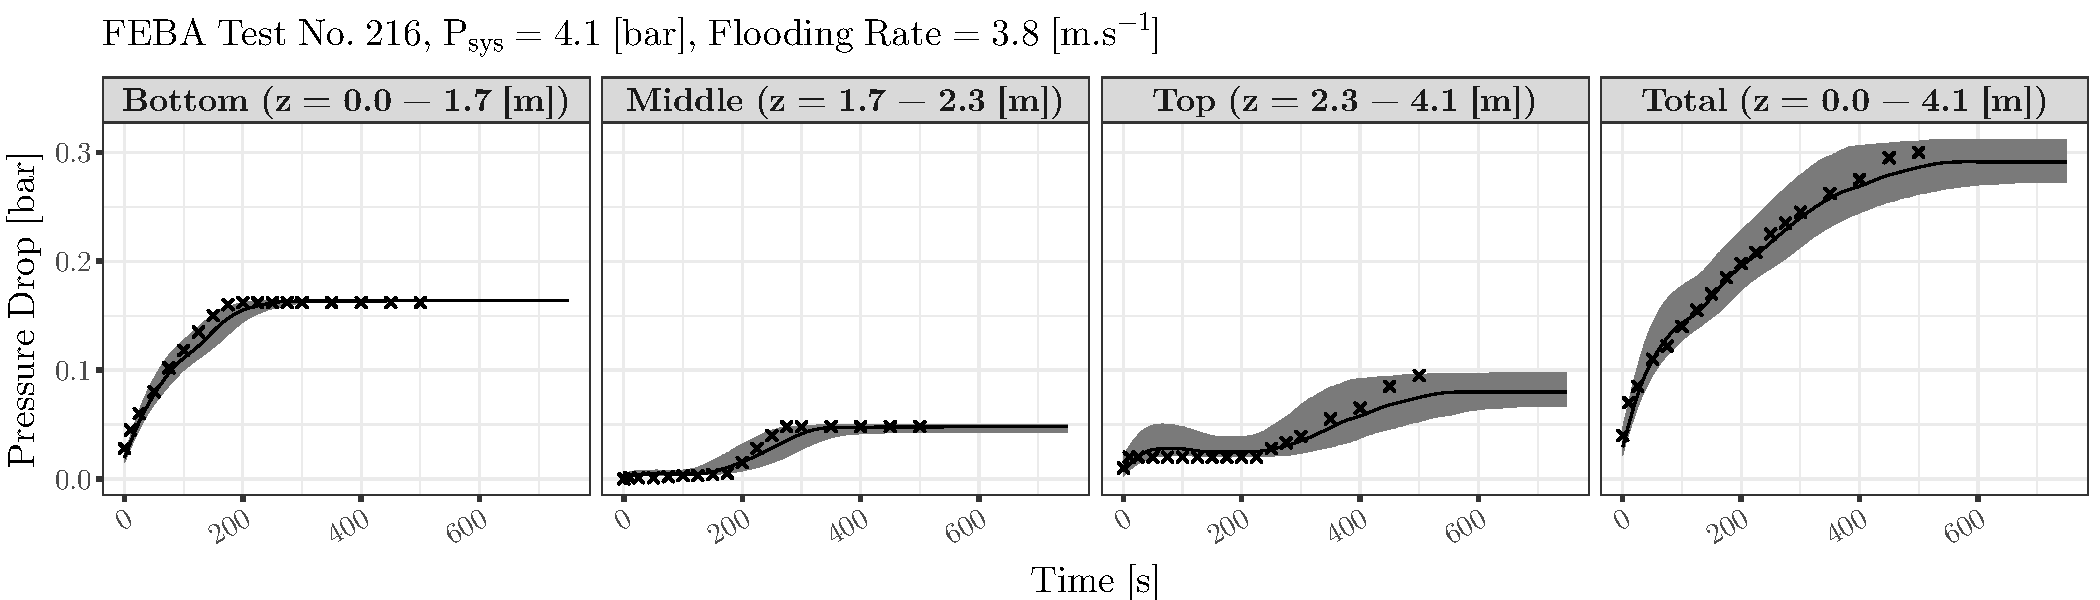
\includegraphics[width=1.0\textwidth]{../figures/chapter2/figures/plotTraceUQPriorDP216}
    \caption[Propagation of the $27$ input parameters prior uncertainties on FEBA test no. $216$ for the pressure drop output ($DP$).]{Propagation of the $27$ input parameters prior uncertainties on FEBA test no. $216$ for the pressure drop output ($DP$). The uncertainty bounds correspond to the symmetric ($95\%$) probability; solid lines and crosses indicate the simulation with the nominal parameters values and the experimental data, respectively.}
    \label{fig:ch2_app_plot_trace_uq_prior_dp_216}
\end{figure}

% FEBA test no. 223 Prior Uncertainty Propagation, DP
\begin{figure}[!h]
    \centering
    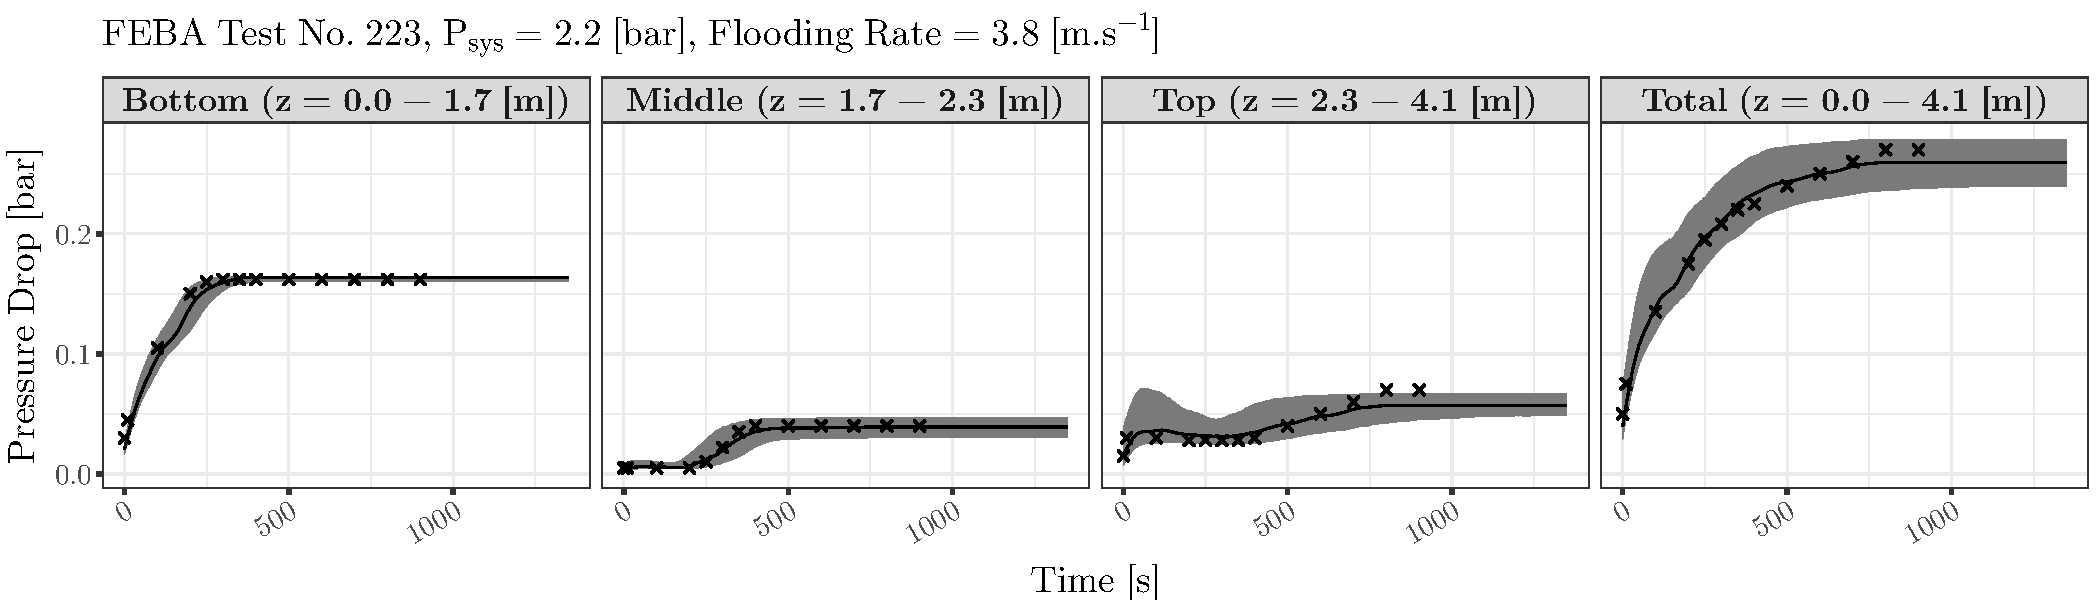
\includegraphics[width=1.0\textwidth]{../figures/chapter2/figures/plotTraceUQPriorDP223}
    \caption[Propagation of the $27$ input parameters prior uncertainties on FEBA test no. $223$ for the pressure drop output ($DP$).]{Propagation of the $27$ input parameters prior uncertainties on FEBA test no. $223$ for the pressure drop output ($DP$). The uncertainty bounds correspond to the symmetric ($95\%$) probability; solid lines and crosses indicate the simulation with the nominal parameters values and the experimental data, respectively.}
    \label{fig:ch2_plot_trace_uq_prior_dp_223}
\end{figure}

\clearpage

% FEBA test no. 218 Prior Uncertainty Propagation, DP
\begin{figure}[bth]
    \centering
    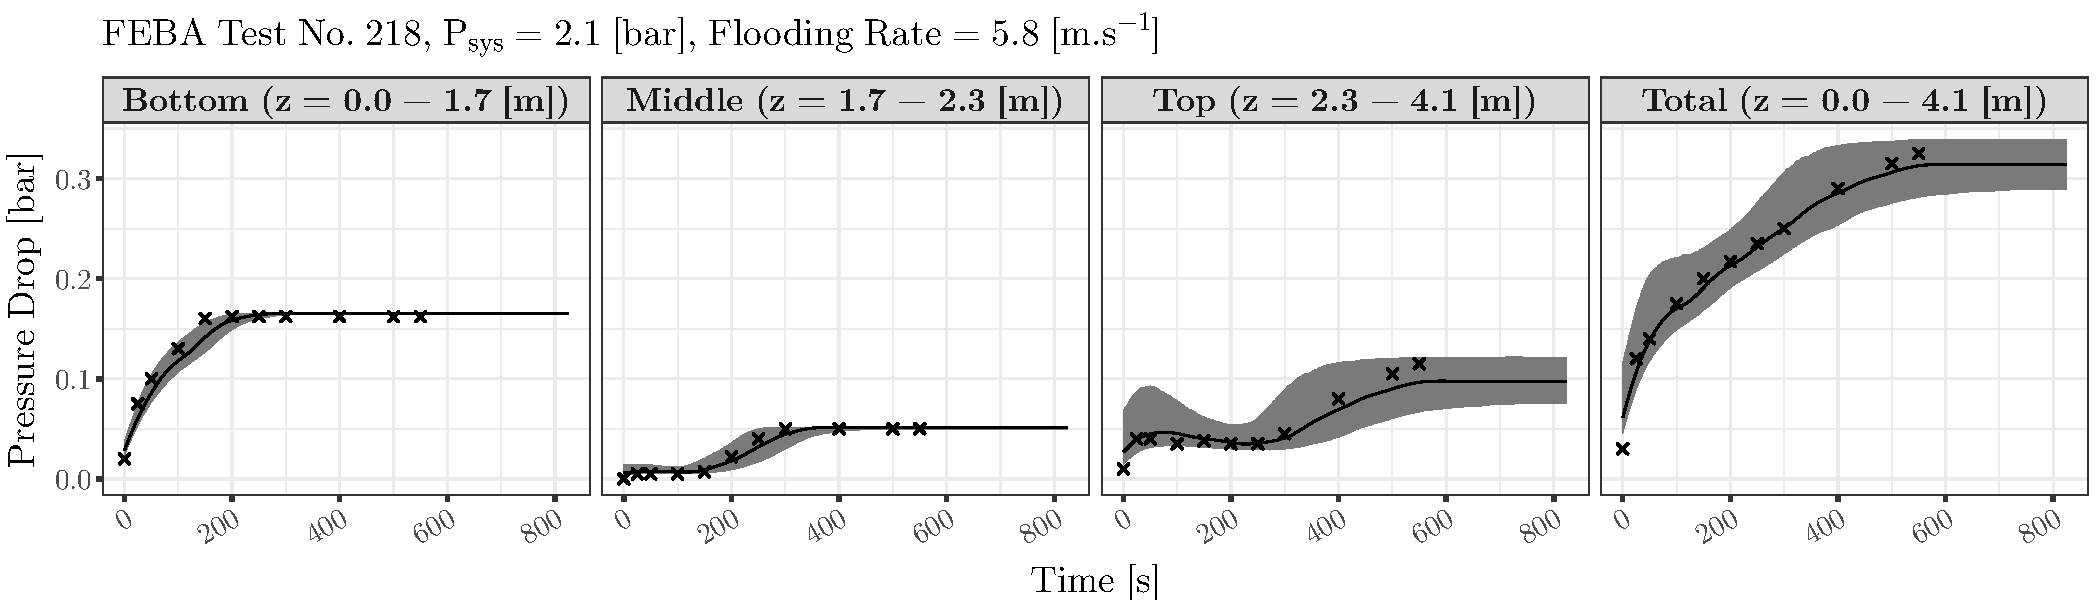
\includegraphics[width=1.0\textwidth]{../figures/chapter2/figures/plotTraceUQPriorDP218}
    \caption[Propagation of the $27$ input parameters prior uncertainties on FEBA test no. $218$ for the pressure drop output ($DP$).]{Propagation of the $27$ input parameters prior uncertainties on FEBA test no. $218$ for the pressure drop output ($DP$). The uncertainty bounds correspond to the symmetric ($95\%$) probability; solid lines and crosses indicate the simulation with the nominal parameters values and the experimental data, respectively.}
    \label{fig:ch2_plot_trace_uq_prior_dp_218}
\end{figure}

% FEBA test no. 220 Prior Uncertainty Propagation, DP
\begin{figure}[bth]
    \centering
    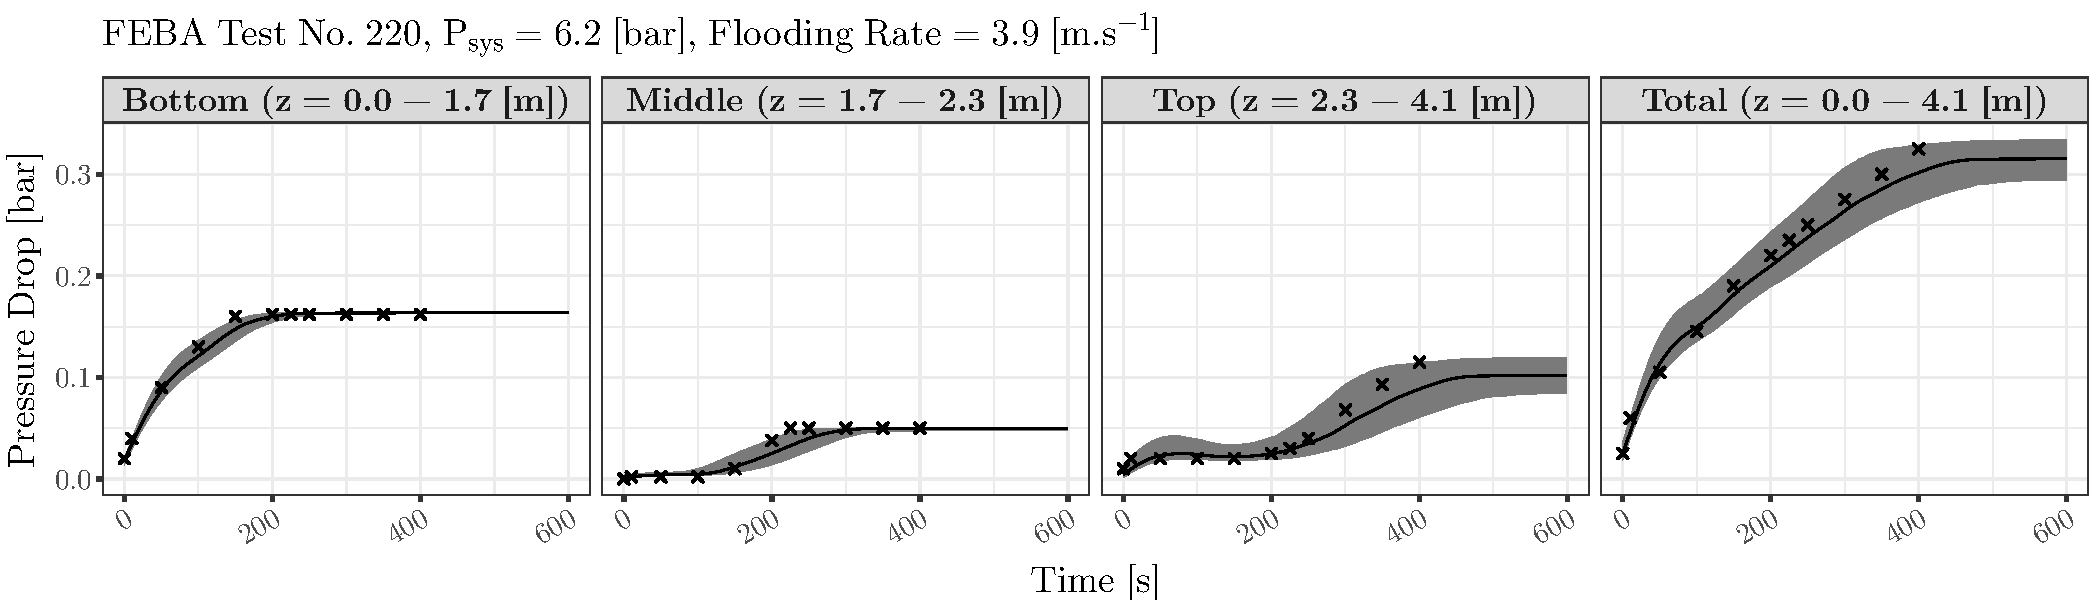
\includegraphics[width=1.0\textwidth]{../figures/chapter2/figures/plotTraceUQPriorDP220}
    \caption[Propagation of the $27$ input parameters prior uncertainties on FEBA test no. $220$ for the pressure drop output ($DP$).]{Propagation of the $27$ input parameters prior uncertainties on FEBA test no. $220$ for the pressure drop output ($DP$). The uncertainty bounds correspond to the symmetric ($95\%$) probability; solid lines and crosses indicate the simulation with the nominal parameters values and the experimental data, respectively.}
    \label{fig:ch2_plot_trace_uq_prior_dp_220}
\end{figure}

% FEBA test no. 222 Prior Uncertainty Propagation, DP
\begin{figure}[!h]
    \centering
    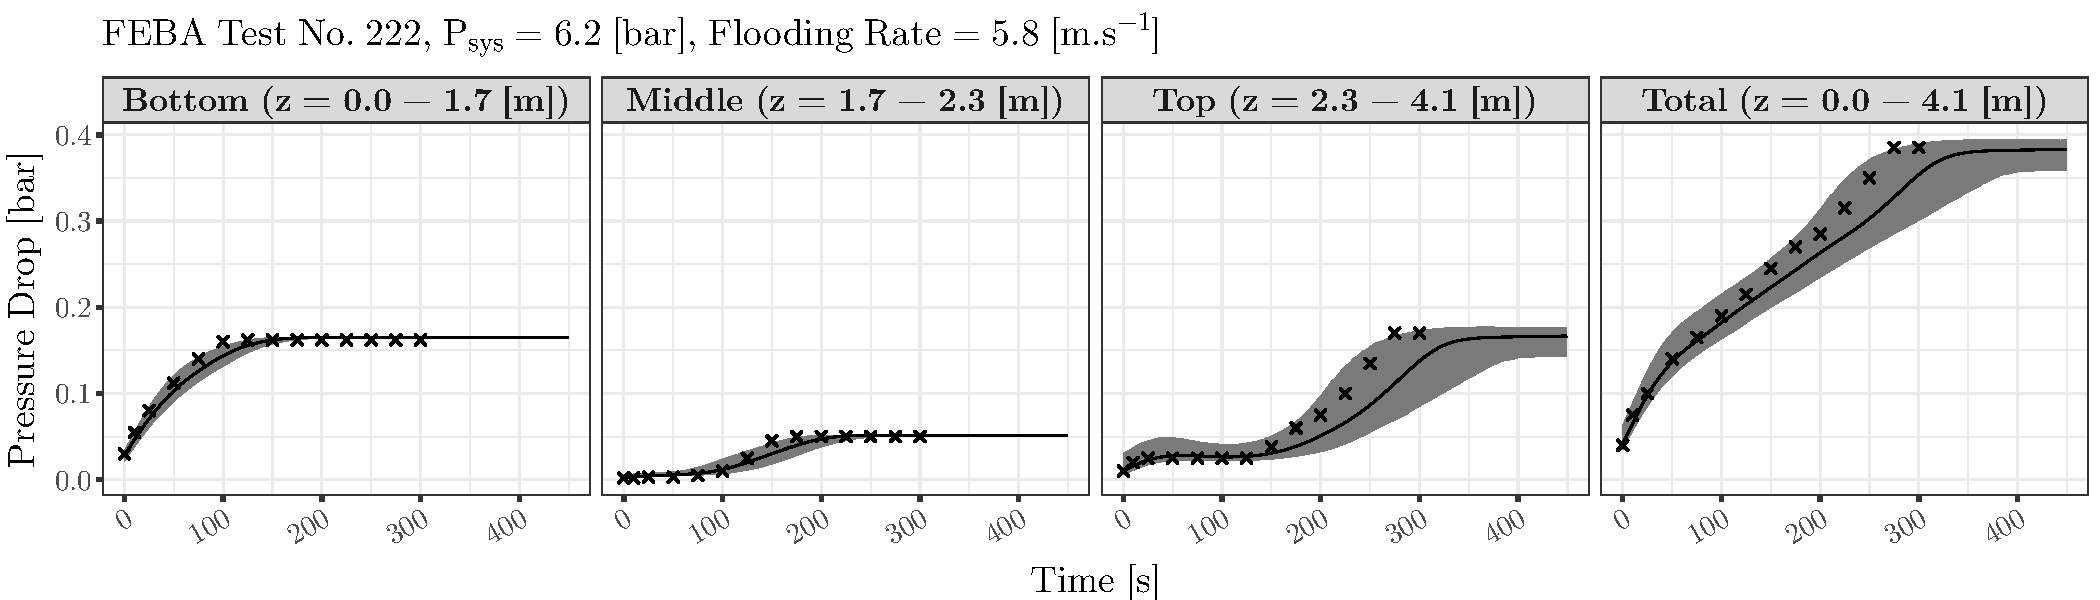
\includegraphics[width=1.0\textwidth]{../figures/chapter2/figures/plotTraceUQPriorDP222}
    \caption[Propagation of the $27$ input parameters prior uncertainties on FEBA test no. $222$ for the pressure drop output ($DP$).]{Propagation of the $27$ input parameters prior uncertainties on FEBA test no. $222$ for the pressure drop output ($DP$). The uncertainty bounds correspond to the symmetric ($95\%$) probability; solid lines and crosses indicate the simulation with the nominal parameters values and the experimental data, respectively.}
    \label{fig:ch2_plot_trace_uq_prior_dp_222}
\end{figure}

\clearpage

%--------------------------------------------------------------------------
\subsection{Liquid carryover Output (CO)}\label{app:tbl_results_uq_feba_co}
%--------------------------------------------------------------------------

% FEBA test no. 214 - 216 Prior Uncertainty Propagation, CO
\normdoublefigure[pos=tbhp,
                  mainlabel={fig:ch2_plot_trace_uq_prior_co_1},
                  maincaption={Propagation of the $27$ input parameters prior uncertainties on FEBA test nos. $214$ \& $218$ for the liquid carryover output ($CO$). The uncertainty bounds correspond to the symmetric ($95\%$) probability; solid lines and crosses indicate the simulation with the nominal parameters values and the experimental data, respectively.},
				mainshortcaption={Propagation of the $27$ input parameters prior uncertainties on FEBA test nos. $214$ \& $218$ for the liquid carryover output ($CO$).},
                  leftopt={width=0.45\textwidth},
                  leftlabel={fig:ch2_plot_trace_uq_prior_co_214},
                  leftcaption={\gls[hyper=false]{feba} test no. $214$},
                  %leftshortcaption={},%
                  rightopt={width=0.45\textwidth},
                  rightlabel={fig:ch2_app_plot_trace_uq_prior_co_216},
                  rightcaption={\gls[hyper=false]{feba} test no. $216$}]
{../figures/chapter2/figures/plotTraceUQPriorCO214}
{../figures/chapter2/figures/plotTraceUQPriorCO216}

% FEBA test no. 223 - 218 Prior Uncertainty Propagation, CO
\normdoublefigure[pos=!h,
                  mainlabel={fig:ch2_plot_trace_uq_prior_co_2},
                  maincaption={Propagation of the $27$ input parameters prior uncertainties on FEBA test nos. $223$ \& $218$ for the liquid carryover output ($CO$). The uncertainty bounds correspond to the symmetric ($95\%$) probability; solid lines and crosses indicate the simulation with the nominal parameters values and the experimental data, respectively.},
				mainshortcaption={Propagation of the $27$ input parameters prior uncertainties on FEBA test nos. $223$ \& $218$ for the liquid carryover output ($CO$).},
                  leftopt={width=0.45\textwidth},
                  leftlabel={fig:ch2_plot_trace_uq_prior_co_223},
                  leftcaption={\gls[hyper=false]{feba} test no. $223$},
                  %leftshortcaption={},%
                  rightopt={width=0.45\textwidth},
                  rightlabel={fig:ch2_plot_trace_uq_prior_co_218},
                  rightcaption={\gls[hyper=false]{feba} test no. $218$}]
{../figures/chapter2/figures/plotTraceUQPriorCO223}
{../figures/chapter2/figures/plotTraceUQPriorCO218}

% FEBA test no. 220 - 222 Prior Uncertainty Propagation, CO
\normdoublefigure[pos=!h,
                  mainlabel={fig:ch2_plot_trace_uq_prior_co_3},
                  maincaption={Propagation of the $27$ input parameters prior uncertainties on FEBA test nos. $220$ \& $222$ for the liquid carryover output ($CO$). The uncertainty bounds correspond to the symmetric ($95\%$) probability; solid lines and crosses indicate the simulation with the nominal parameters values and the experimental data, respectively.},
				mainshortcaption={Propagation of the $27$ input parameters prior uncertainties on FEBA test nos. $220$ \& $222$ for the liquid carryover output ($CO$).},
                  leftopt={width=0.45\textwidth},
                  leftlabel={fig:ch2_plot_trace_uq_prior_co_220},
                  leftcaption={\gls[hyper=false]{feba} test no. $220$},
                  %leftshortcaption={},%
                  rightopt={width=0.45\textwidth},
                  rightlabel={fig:ch2_plot_trace_uq_prior_co_222},
                  rightcaption={\gls[hyper=false]{feba} test no. $222$}]
{../figures/chapter2/figures/plotTraceUQPriorCO220}
{../figures/chapter2/figures/plotTraceUQPriorCO222}

\clearpage